

% Assumption which should also be mentioned in a preceding section: transmission range circular and of equal size.

\section{Redundancy reduction of distance-to-contour flooding}\label{sec:contri2}

Broadcasting information from a source user to the rest of the network with regular flooding causes problems such as redundancy, contention and collisions \cite{storm}. Redundant messages also unnecessarily increase the interference.  The distance-to-contour flooding algorithm reduces the number of flooding messages by using a back-off timer to impose an ordering on the transmitting users. For a network with $n$ users, the number of flooding messages is approximately equal to $n$. In this section we propose an alternative to DTC that reduces the number of transmitting users further. From now on, we refer to the adapted distance-to-contour flooding algorithm as the DTC2 flooding algorithm. 

Flooding algorithms can be divided into three categories based on the amount of information users needs from their neighbors \cite{1hopflooding}. The first category are the flooding algorithms that require no information, for example \textit{regular} flooding and \textit{probabilistic} flooding. Algorithms from the second category reduce redundant transmissions by having every user select only a subset of its neighbors to forward a message. For this, a user needs information about his \textit{one-hop} (direct) neighbors. DTC2 belongs to this category. Another example can be found in the work of Liu et.al. \cite{1hopflooding}. The third category contains algorithms that use information about neighbors that are \textit{two hops} or more away \cite{2hop}. 

\subsection{Ideal network topology}

DTC2 selects the forwarding neighbors according to the selection criterium proposed by Hur et. al. \cite{dtc2}. The idea is to approximate an ideal network topology where the overlapping area of the users' transmission ranges is minimized. Fig.~\ref{fig:threeforwards} and Fig.~\ref{fig:fourforwards} show the ideal topology for a user with respectively three and four neighbors and Fig.~\ref{fig:hextiling} and Fig.~\ref{fig:squaretiling} show the resulting hexagonal and square tiling topology in a network. We chose to investigate the square tiling topology from Fig.~\ref{fig:fourforwards} because there is less redundancy in the communication when a user only forwards to four neighbors instead of six neighbors in the hexagonal tiling topology.

In a real network the users are deployed randomly and previous discussed topologies do not occur, so the criterium to select forwarding neighbors is to choose the neighbors located closest to the ideal positions. By reducing the number of forwarding neighbors, the number of transmissions and collisions is also reduced. By choosing the users closest to the ideal positions we aim to have all users in the network receive updates. We express this in terms of the \textit{delivery ratio}, which is the ratio of the number of users that receive flooding messages to the total number of users in the network.

\begin{figure}
\centering
\subfloat[]{\label{fig:threeforwards}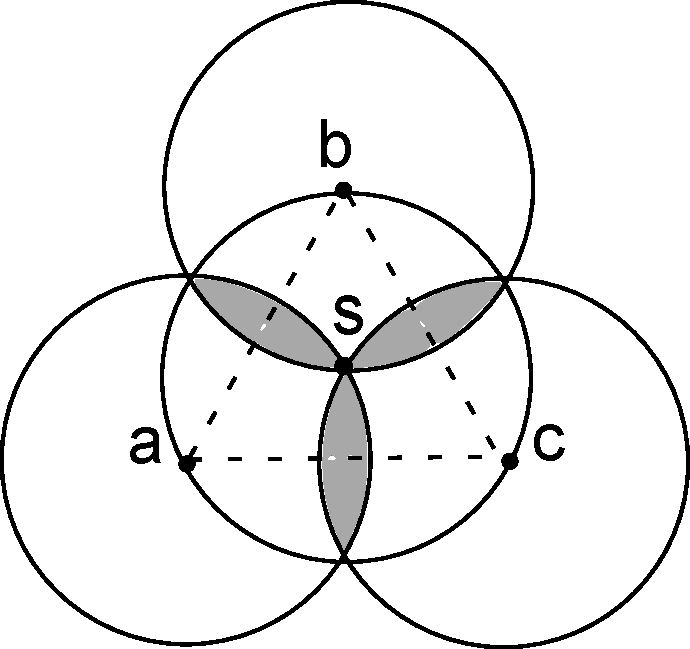
\includegraphics[scale=0.25]{figures/contribution2/threeForwarding.pdf}} \hspace{8mm}
\subfloat[]{\label{fig:fourforwards}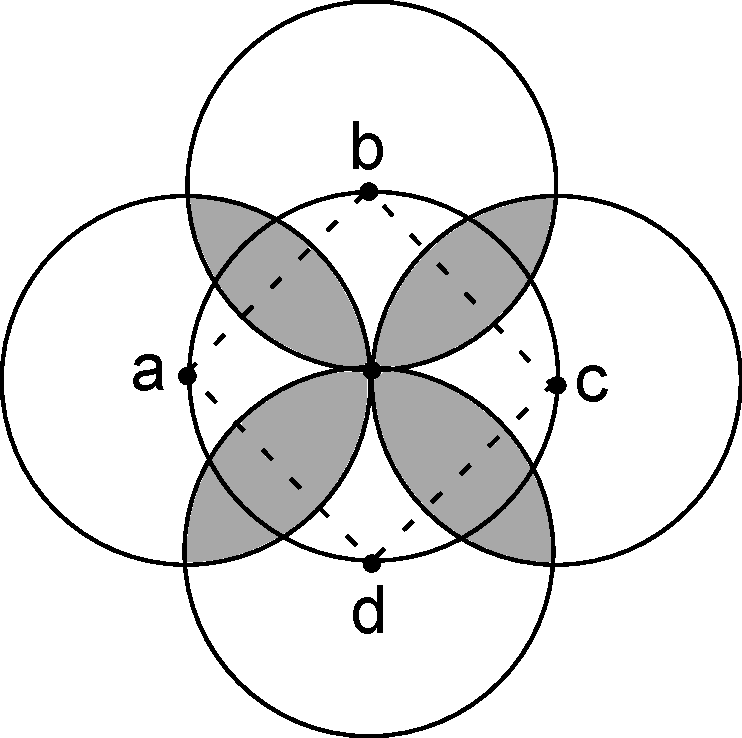
\includegraphics[scale=0.26]{figures/contribution2/fourForwarding.pdf}}  \\ \hspace{3mm}
\subfloat[]{\label{fig:hextiling}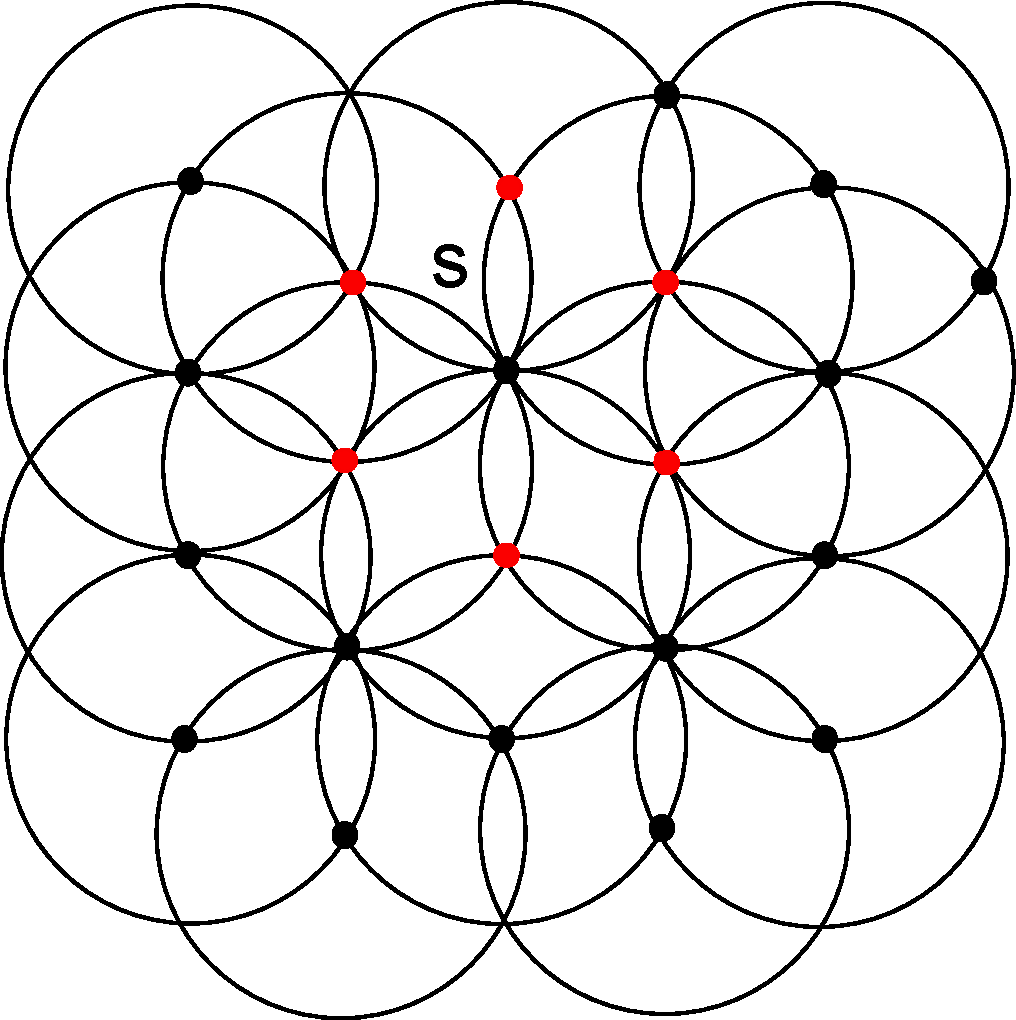
\includegraphics[scale=0.17]{figures/contribution2/hexagonalTiling.pdf}} \hspace{8mm}
\subfloat[]{\label{fig:squaretiling}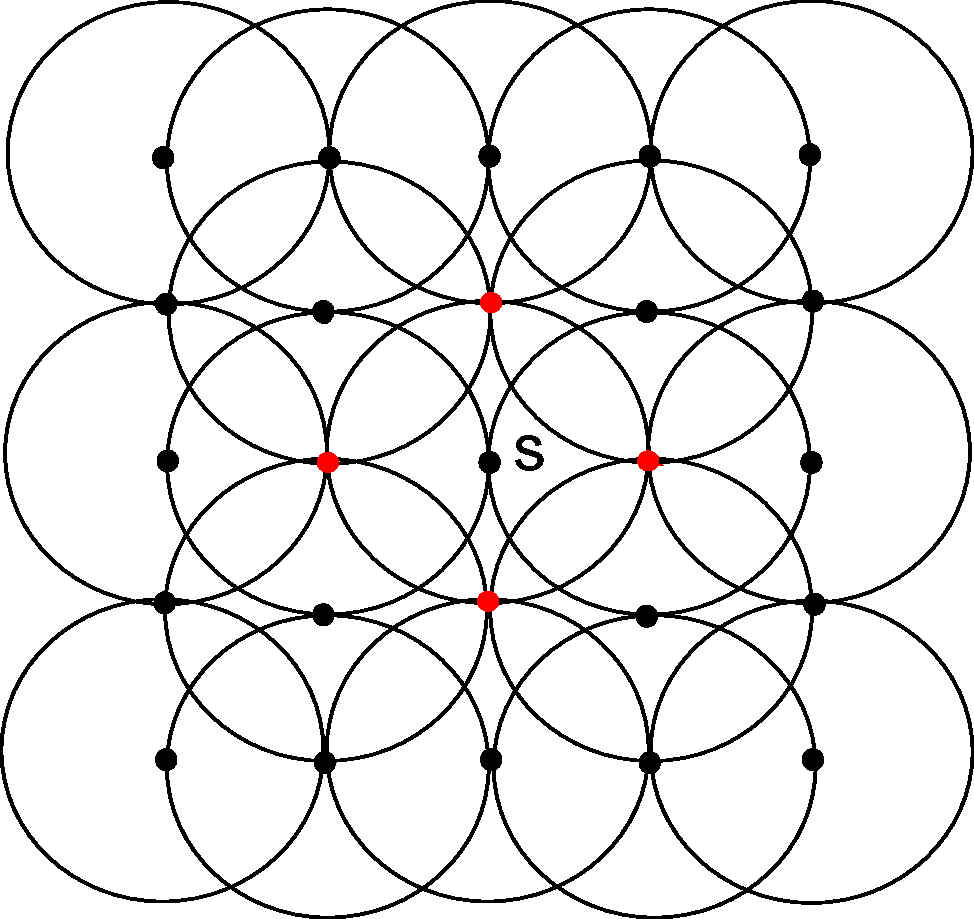
\includegraphics[scale=0.21]{figures/contribution2/squareTiling.pdf}}
\caption{\label{fig:forwarding}Fig.~\ref{fig:threeforwards} and Fig.~\ref{fig:fourforwards} show the ideal topology for a user with respectively three and four neighbors. This topology minimizes the overlapping areas of the transmission ranges. Fig.~\ref{fig:hextiling} and Fig.~\ref{fig:squaretiling} show the resulting network topologies for respectively three and four neighbors. Figures by Hur et. al. \cite{dtc2} }
\end{figure}
% Square tiling is zeer vreemd, check dit nog eens !!!! extra cirkel overal toevoegen in b en d , lost probleem op

\subsection{Forwarding user selection}\label{subsec:forwardingSel}

The procedure to select forwarding neighbors is described by Hur et. al. \cite{dtc2} as follows:

We assume every user knows his position by GPS or a positioning algorithm. Consider user $s$ from Fig.~\ref{fig:partitioning} with co\"ordinates $(x_S,y_S)$. Partitions $P_0,P_1,P_2$ and $P_3$ divide the transmission range of $s$ in four as illustrated in Fig.~\ref{fig:partitioning1}. 

\begin{figure}
\centering
\subfloat[]{\label{fig:partitioning1}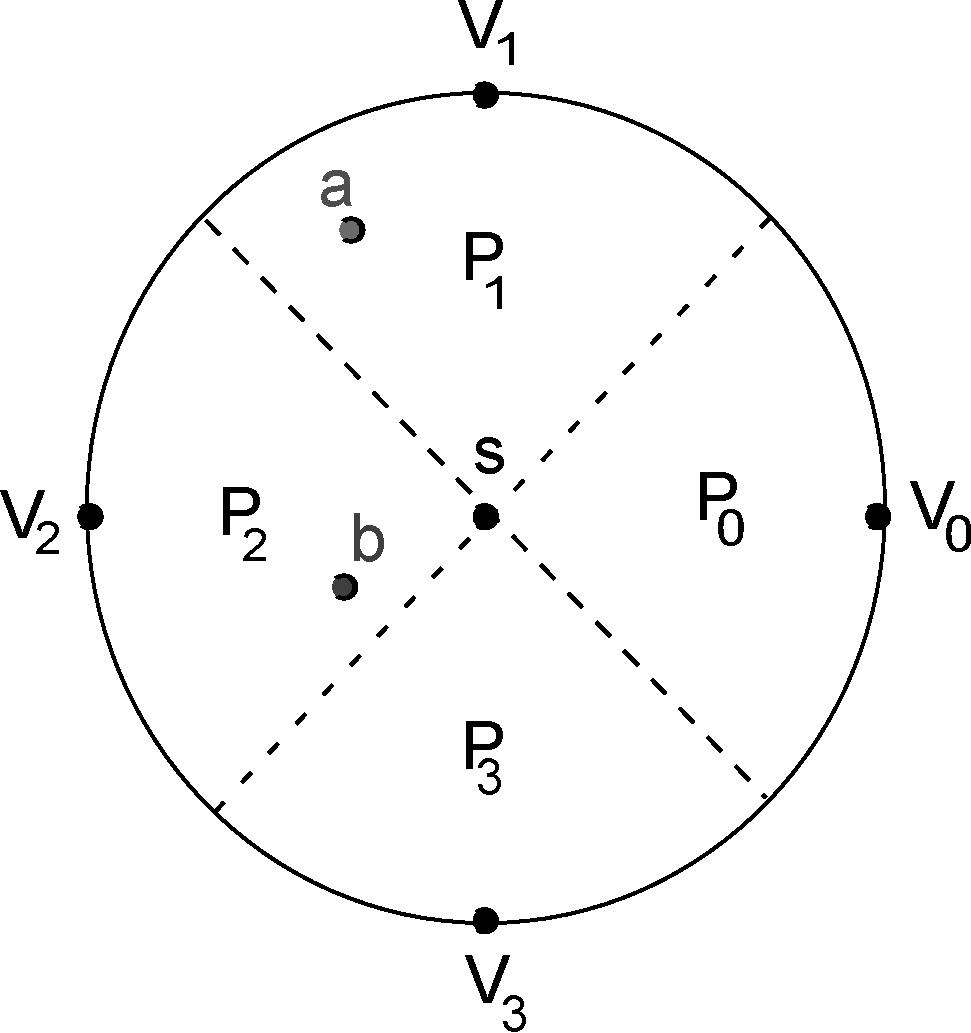
\includegraphics[scale=0.2]{figures/contribution2/partitioning.pdf}} \hspace{6mm}
\subfloat[]{\label{fig:partitioning2}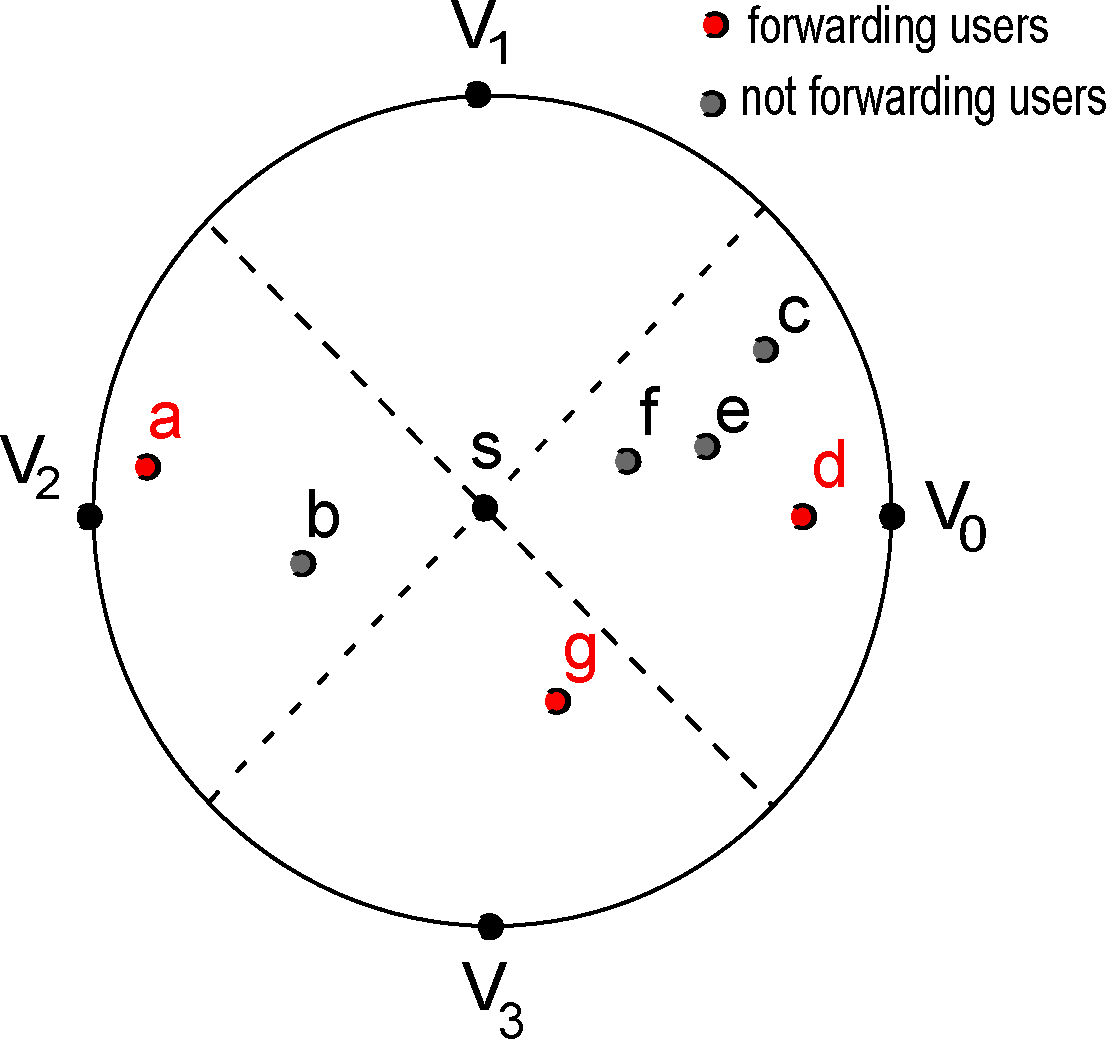
\includegraphics[scale=0.2]{figures/contribution2/userSelection.pdf}}
\caption{\label{fig:partitioning}Fig.~\ref{fig:partitioning1} demonstrates the partitioning of the transmission range of user $s$. Fig.~\ref{fig:partitioning2} shows an example of which users are selected as forwarding neighbors. Figures by Hur et. al. \cite{dtc2}}
\end{figure}

With every partition $P_i$ there is one vertex $V_i$ associated, with $0\leq i\leq3$. These vertices indicate the positions of the four forwarding neighbors in case of an ideal square tiling topology. A user determines the forwarding neighbors as follows: For each partition $P_i$ the neighbor closest to $V_i$ is selected. If the partition is empty, no neighbor is selected. The selection is illustrated in Fig.~\ref{fig:partitioning2}.

Whereas in step three of the DTC algorithm, all the neighbors of a user forward their footpoint, in DTC2 only a subset of forwarding neighbors is selected. We consider again a scenario with transmitter P and $n$ wireless users and describe this third step of DTC2 in which a user $N$ updates his one-hop neighbors about his footpoint $f_N=x_A$. Based on this information the neighbors of $N$ update their footpoint and distance in the same way as in the DTC flooding algorithm. user $N$ also computes the set of forwarding neighbors $F(N)$ as discussed above. 

Consider the following example of the update and forwarding process for a neighbor of user $M$ that is a neighbor of user $N$. User $N$ has footpoint $f_N=x_A$ and distance $d(x_N,x_A)$ to this footpoint. User $M$ has footpoint $f_M=x_B$ and distance $d(x_M,x_B)$ to this footpoint. There are two possibilities:

\begin{enumerate}
\item If $d(x_M,x_A) < d(x_M,x_B)$, then $f_j \leftarrow x_A$ and $d(x_M,f_M) \leftarrow d(x_M,x_B)$. 
	\begin{itemize}
	\item If user $M \not\in F(N)$, $M$ is not added to the queue.
	\item Otherwise, $M$ is added to the queue.
	\end{itemize}
\item If $d(x_M,x_A) \geq d(x_M,x_B)$, then the footpoint of $M$ does not change and user $M$ is not added to the queue, independent of whether it is a member of $F(N)$.
\end{enumerate}
 
\subsection{Simulation results}


\begin{figure*}[!b]
\centering 
\subfloat[]{\label{fig:dtc2nbSends}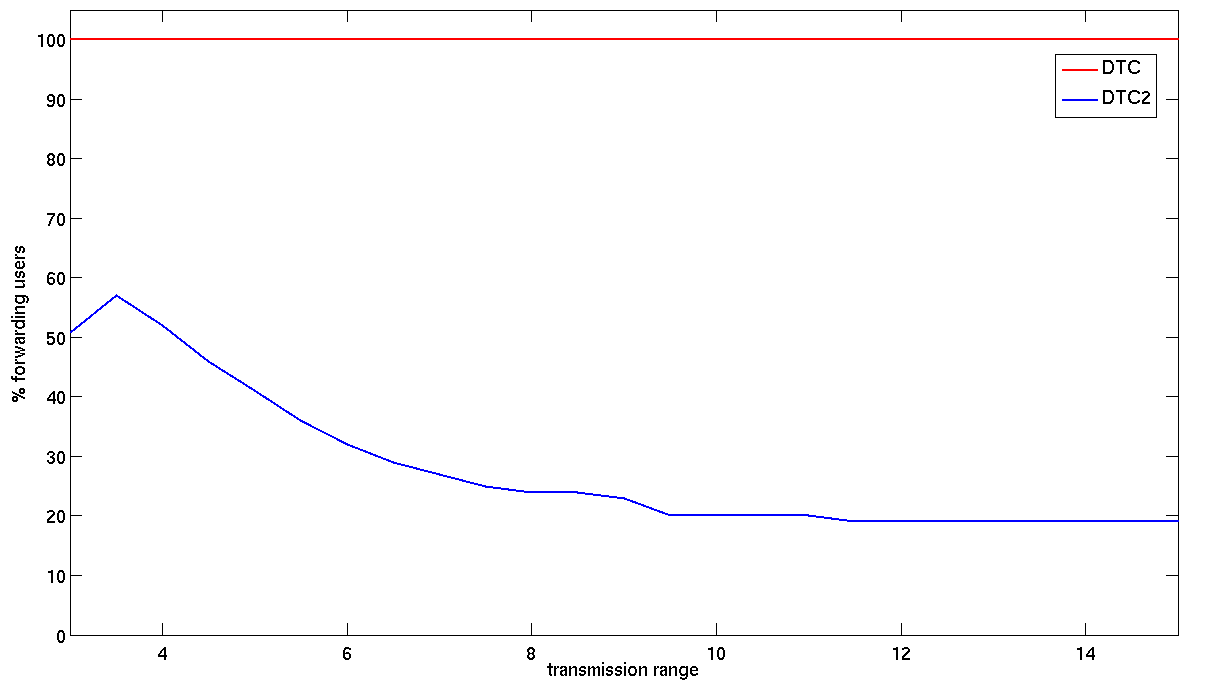
\includegraphics[scale=0.16]{figures/contribution2/nbSends2}} \hspace{1cm}
\subfloat[]{\label{fig:dtc2locprob}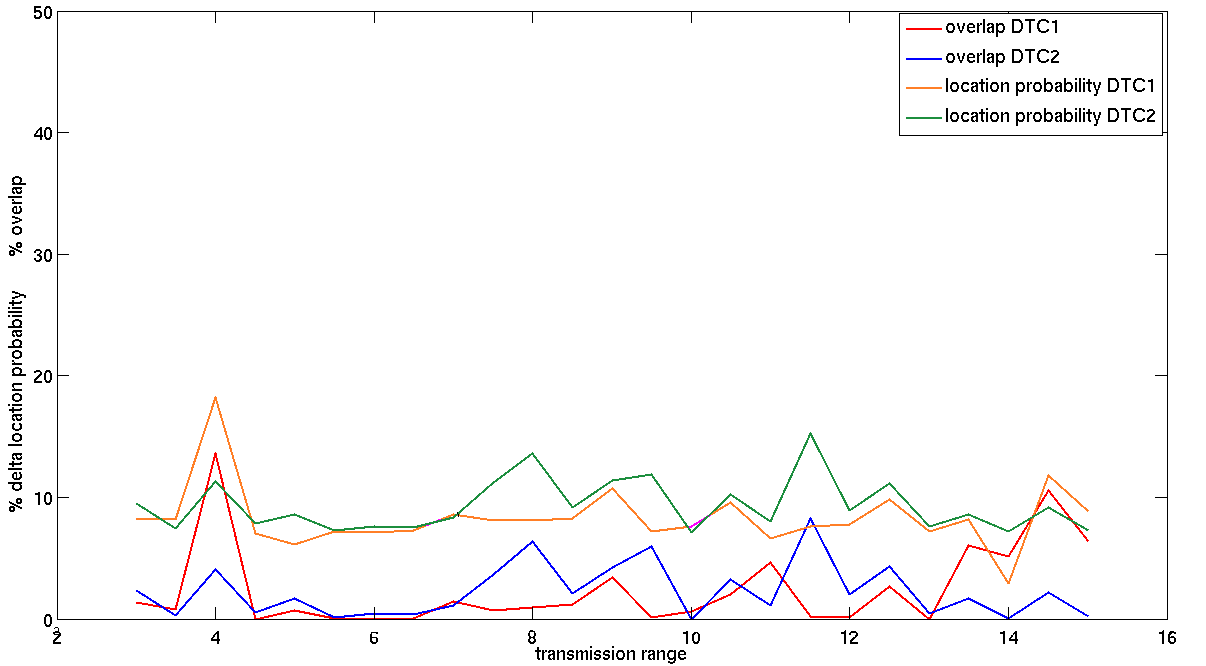
\includegraphics[scale=0.27]{figures/contribution2/locproboverlap2}} \\
\subfloat[]{\label{fig:dtc2misclass}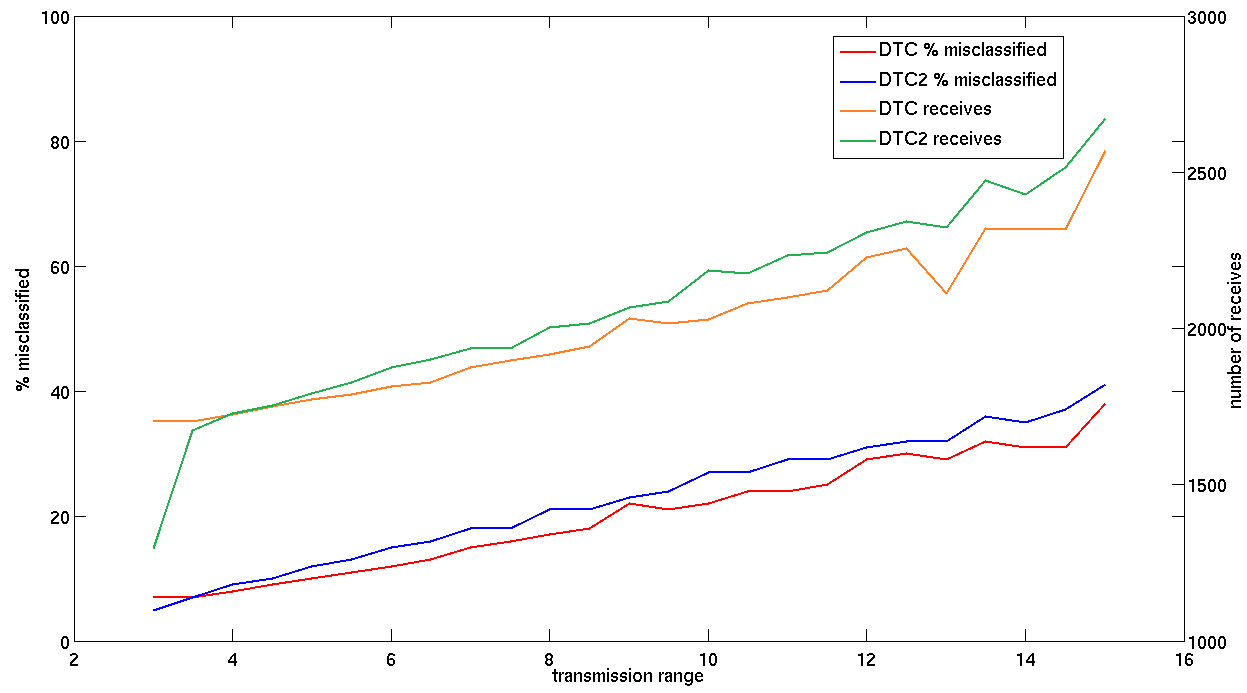
\includegraphics[scale=0.26]{figures/contribution2/misclassified2}}\hspace{1cm}
\subfloat[]{\label{fig:dtc2error}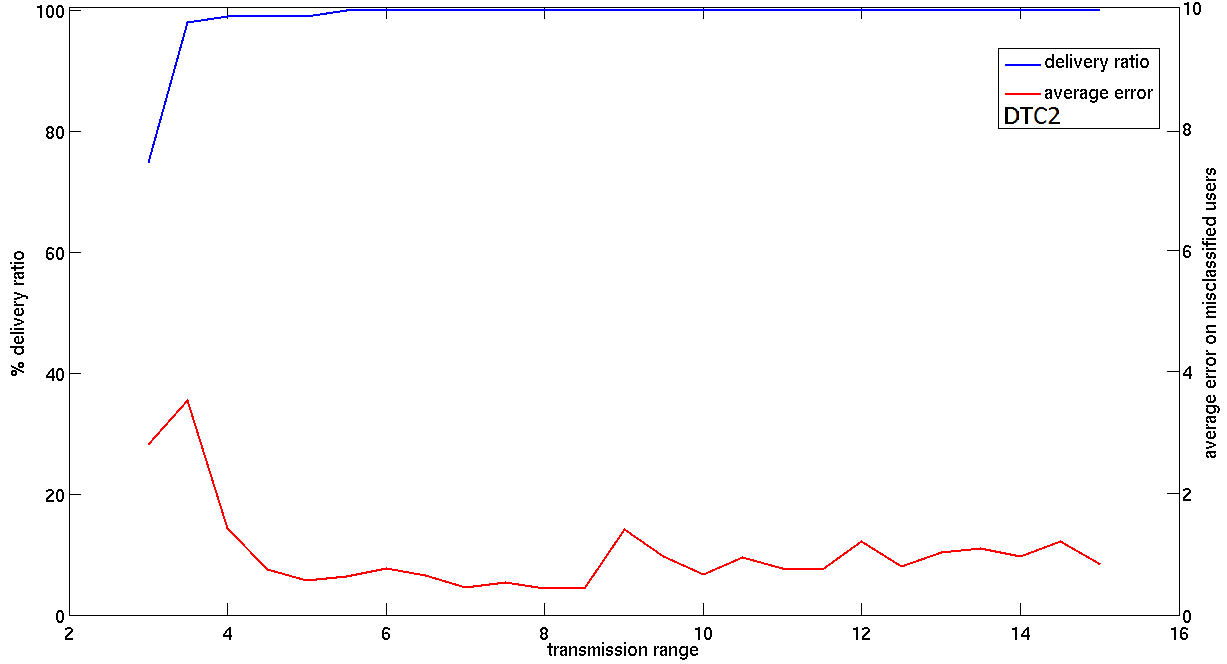
\includegraphics[scale=0.26]{figures/contribution2/error2}}
\caption{Fig.~\ref{fig:dtc2nbSends}: The percentage of forwarding users for DTC2 in comparison with the number of forwarding users for DTC. Fig.~\ref{fig:dtc2locprob}: Percentage overlap of the primary contour by the secondary contour together with the percentage reduction of the $95\%$ location probability contour of the primary transmitter in comparison with the absence of a secondary transmitter. Fig.~\ref{fig:dtc2misclass}: Percentage of misclassified users and number of receives (or updates) for DTC and DTC2. Fig.~\ref{fig:dtc2error}: The average error on the distance to footpoint for the DTC2 algorithm together with the delivery ratio.}
\end{figure*}

In this section we compare some performance metrics for simulations of the IPA algorithm with both DTC and DTC2. We look at the communication redundancy in terms of the size of the transmission range (also called communication range) and investigate whether using DTC2 has an influence on the reliability of the computation of the power of the secondary transmitter. The results are averages over three simulations. For DTC, all the users forward information and the transmission range has no influence. For DTC2, an increase in the transmission range reduces the percentage of forwarding users, as shown in Fig.~\ref{fig:dtc2nbSends}. This is because the number of forwarding neighbors per user is always maximum. However, in comparison with DTC, extra communication is needed to inform a user about the positions of his neighbors. A user needs this information to determine the forwarding set of neighbors. 

For a network with $n$ users, the number of updates for the DTC algorithm is slightly larger than $n$ because of collisions and misclassified users, as explained in section \ref{sec:dtc1}. Fig.~\ref{fig:dtc2misclass} shows the percentage of misclassified users and the number of updates in function of the kernel width. In the simulated network, the users are randomly distributed and the topology is not ideal. Therefore not all users receive their correct footpoint when using DTC2 and the number of misclassified users is slightly larger than for DTC. However, the incorrect footpoint is always received from a user within the distance of a one-hop neighbor so the error is not large. Fig.~\ref{fig:dtc2error} shows that the average error is never larger than $3\%$. It seems that as the transmission range increases, the average error also slightly increases, but this should be investigated further. When the delivery ratio is smaller than one, because the transmission range is too small, the average error increases as shown in Fig.~\ref{fig:dtc2error}. 

Last, Fig.~\ref{fig:dtc2locprob} shows that using DTC2 does not have an effect on the performance of the IPA algorithm. The size of the transmission range also has no influence. We see no difference in the size of the overlap of the contours or the reduction of the location probability when using DTC or DTC2, or by varying the transmission range. We also investigated that the number of iterations for the IPA algorithm to converge lies between three and seven iterations, regardless of whether DTC or DTC2 is used.


